\section{Introduction}\label{sec:intro}

The almost Mathieu operator
\begin{equation}\label{eq:amo}
(H_{\lambda,\alpha,\theta}u)(n)=u(n+1)+u(n-1)+2\lambda\cos\bigl(2\pi(\theta+n\alpha)\bigr)u(n)
\end{equation}
on $\ell^2(\Z)$ is the central model of quasi-periodic spectral theory. Physicists know it as the Aubry--Andr\'e model~\cite{AubryAndre1980}, and it is realized with cold atoms in bichromatic optical lattices~\cite{Roati2008} and with light in quasi-periodic waveguide arrays~\cite{Lahini2009}. Here $\lambda>0$ is the coupling, $\alpha$ is an irrational frequency and $\theta\in\T=\R/\Z$ is a phase. For $\lambda>1$ the Lyapunov exponent on the spectrum equals $\log\lambda>0$~\cite{BourgainJitomirskaya2002}, but positivity alone does not imply localization.

That picture depends on the arithmetic of $\alpha$. Let $p_n/q_n$ be the continued-fraction convergents of $\alpha$ and
\begin{equation}\label{eq:beta}
\beta(\alpha)=\limsup_{n\to\infty}\frac{\log q_{n+1}}{q_n}\in[0,\infty].
\end{equation}
Avila, You and Zhou~\cite{AYZ2017} proved that the supercritical regime splits sharply at $\lambda=e^{\beta(\alpha)}$. For $\lambda>e^{\beta}$ the operator has Anderson localization for almost every phase. For $1<\lambda<e^{\beta}$ the spectrum is purely singular continuous for every phase. Strongly Liouville frequencies, those with $\beta(\alpha)>0$, can therefore destroy localization even though the Lyapunov exponent stays positive.

What does a wave packet do in that window? For almost every phase, we determine every upper Abel-averaged transport moment exponent and both packing dimensions of every nonzero spectral measure; they equal the same number. The matching lower bounds hold at every phase. The word \emph{upper} matters: the exponent describes the largest long-time bursts, not a power law valid at every time.

The main conclusions are easy to separate. First, the competition between $\log\lambda$ and $\beta(\alpha)$ gives an exact upper transport law on the phase set of Theorem~\ref{thm:A}; when $\beta(\alpha)>\log\lambda$, almost all of the Abel-averaged packet reaches the radii and times specified in Theorem~\ref{thm:B}, at every phase. Second, the same law determines packing dimensions under Theorem~\ref{thm:C}'s phase conditions and, for a packet started at one site, the upper generalized R\'enyi dimensions of orders $0<r<1$ under Theorem~\ref{thm:renyi}'s phase conditions. Third, a computable frequency can produce a noncomputable exponent even though finite-time probabilities for computable data remain effectively approximable. This computability degree persists under computable changes of coupling in an interval; at coupling $2$ and phase $1/4$, however, any finite frequency prefix and any nonzero finite-time error tolerance permit every exponent in the class of Theorem~\ref{thm:D}(2).

\subsection{Transport exponents}

Let $\psi_t=e^{-itH}\delta_0$ and average in time with the exponential weight $(2/T)e^{-2t/T}$:
\begin{equation}\label{eq:abel}
a(j,T)=\frac2T\int_0^\infty e^{-2t/T}\,|\langle\delta_j,\psi_t\rangle|^2\,dt,\qquad
P(N,T)=\sum_{|j|>N}a(j,T),\qquad M_p(T)=\sum_{j\in\Z}|j|^p a(j,T).
\end{equation}
$P(N,T)$ is the time-averaged probability of finding the particle beyond distance $N$, and $M_p(T)$ is the averaged $p$-th moment of the position. The upper transport exponents are
\begin{equation}\label{eq:exponents}
\beta^+(p)=\limsup_{T\to\infty}\frac{\log M_p(T)}{p\log T},\qquad
\au=\sup_{p>0}\beta^+(p).
\end{equation}
The quantity $\au$ is the fastest upper exponent of Damanik and Tcheremchantsev~\cite{DT2007}. It sees even polynomially small tails: if $P(T^a,T)$ decays faster than every power of $T$, then $\au\le a$; if $P(T_j^a,T_j)\ge cT_j^{-C}$ for some $c>0$, $C<\infty$ and a sequence $T_j\to\infty$, then $\au\ge a$. Always $0\le\au\le1$, since hopping is bounded.

Two endpoints were known. Damanik and Tcheremchantsev proved $\au=0$ for $\lambda>1$ when $\beta(\alpha)=0$~\cite{DT2007}, and Jitomirskaya and Zhang proved $\au=1$ for every phase when $\beta(\alpha)=\infty$~\cite{JZ2022}. Jitomirskaya and Kr\"uger proved exponential dynamical localization in phase expectation when $\beta(\alpha)$ is sufficiently small, including positive values~\cite{JK2013}, and Bradshaw, de Jong, Liu, Wang, Wang and Yang refined the growth rates for weakly Liouville frequencies with $\beta(\alpha)=0$~\cite{BdJLWWY2025}. In between, Jitomirskaya and Zhang obtained lower bounds of the form $1-C\log\lambda/\beta$, for every moment~\cite{JZ2022}. Haeming refined them, with an explicit constant, a logarithmic loss and one sequence of times common to all phases~\cite{Haeming2025}. Upper bounds on fractal dimensions of spectral measures near the transition were obtained by Jitomirskaya, Liu and Tcheremchantsev~\cite{JLT2025}. The exact value was open.

\subsection{Main results}

For the exact upper law we use an explicit full-measure set of phases. Begin with
\begin{equation}\label{eq:Ga}
\Ga=\bigl\{\theta\in\T:\ |\sin(2\pi q_n\theta)|\ge q_n^{-2}\ \text{for all sufficiently large }n\bigr\}.
\end{equation}
This set has full Lebesgue measure for every irrational $\alpha$ (Lemma~\ref{lem:Ga}). We shall in fact work with the larger set
\begin{equation}\label{eq:Gastar}
\Ga^*=\Bigl\{\theta\in\T:\ \begin{array}{l}
\text{for every }c,\zeta>0\text{ there is }n_0\text{ such that}\\
|\sin(2\pi q_n\theta)|\ge e^{-\zeta q_n}
\text{ whenever }n\ge n_0\text{ and }b_n\ge c
\end{array}\Bigr\}.
\end{equation}
Here $b_n$ is defined in Section~\ref{sec:prelim}; a condition on a finite set of indices is vacuous, so $\Ga^*=\T$ when $\beta(\alpha)=0$. Equivalently, for every $c>0$ such that $b_n\ge c$ for infinitely many $n$, $q_n^{-1}\log|\sin(2\pi q_n\theta)|\to0$ along those $n$, with $\log0=-\infty$. Only scales with $b_n\ge c$ enter, and along them $|\sin(2\pi q_n\theta)|$ may tend to zero at any subexponential rate. The complement of $\Ga^*$ contains the set $\frac12(\Z+\alpha\Z)$ of phases at which $H_{\lambda,\alpha,\theta}$ is reflection symmetric whenever $\beta(\alpha)>0$, in particular $\theta=0$ (Lemma~\ref{lem:Gastar}). Throughout, the number $\max\{0,1-\log\lambda/\beta(\alpha)\}$ is read as $0$ when $\beta(\alpha)=0$ and as $1$ when $\beta(\alpha)=\infty$.

\begin{maintheorem}[The transport law]\label{thm:A}
Let $\lambda>1$ and let $\alpha$ be irrational.
\begin{enumerate}
\item If $\beta(\alpha)<\infty$, then for every $\theta\in\Ga^*$ and every $p>0$,
\[
\beta^+(p)=\au=\max\Bigl\{0,\ 1-\frac{\log\lambda}{\beta(\alpha)}\Bigr\}
\]
for $H_{\lambda,\alpha,\theta}$, where the right side is read as $0$ when $\beta(\alpha)=0$.
Moreover, for every $a>\max\{0,1-\log\lambda/\beta(\alpha)\}$ and every $m>0$, $P(T^a,T)=O(T^{-m})$ as $T\to\infty$.
\item If $\beta(\alpha)=\infty$, then $\beta^+(p)=\au=1$ for every phase and every $p>0$.
\end{enumerate}
The lower bound $\beta^+(p)\ge\max\{0,1-\log\lambda/\beta(\alpha)\}$ in part~1 holds for every phase and every $p>0$.
\end{maintheorem}

Part~2 is due to Jitomirskaya and Zhang~\cite[Corollary~3]{JZ2022}, and the case $\beta(\alpha)=0$ of part~1 to Damanik and Tcheremchantsev~\cite{DT2007}; we include them so that the statement covers every frequency. The new content is part~1 for $0<\beta(\alpha)<\infty$: the upper bound throughout, and the matching lower bound for every moment when $\beta(\alpha)>\log\lambda$. For $0<\beta(\alpha)<\infty$, the lower bound for the fastest exponent $\au$ also holds for a Lipschitz sampling function whose Lyapunov exponent is continuous on a neighborhood of a spectral minimizer, with $\log\lambda$ replaced by that minimum (Theorem~\ref{thm:L}).

For $\beta(\alpha)<\infty$ and $\theta\in\Ga^*$, Theorem~\ref{thm:A} identifies the competition between the localization rate $\log\lambda$ and the arithmetic rate $\beta(\alpha)$. If $0<\beta(\alpha)<\infty$, the common upper exponent is zero for $\lambda\ge e^{\beta(\alpha)}$, including equality, and increases continuously to $1$ as $\lambda\downarrow1$. If $\beta(\alpha)=0$, it is zero for every $\lambda>1$; if $\beta(\alpha)=\infty$, it is $1$ for every $\lambda>1$ and every phase. Thus, at almost every phase, the finite-positive-beta spectral transition of~\cite{AYZ2017} is also a sharp transition for upper transport exponents. Figure~\ref{fig:exponent} plots the law.

\begin{figure}[t]
\centering
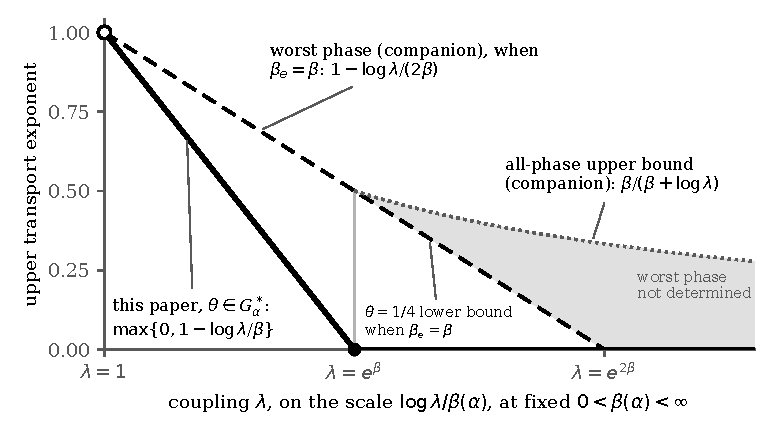
\includegraphics[width=0.8\textwidth]{fig_exponent.pdf}
\caption{The exponent picture: a plot of proved formulas, not of numerical data. At a fixed $0<\beta(\alpha)<\infty$ the horizontal coordinate is $\log\lambda/\beta(\alpha)$, so the marked points are $\lambda=1$, $e^{\beta(\alpha)}$ and $e^{2\beta(\alpha)}$. Solid line: the law of this paper, $\max\{0,1-\log\lambda/\beta(\alpha)\}$, which for $\theta\in G_\alpha^*$ is the common value of every upper Abel-averaged transport exponent and of both packing dimensions of every nonzero spectral measure (Theorems~\ref{thm:A} and~\ref{thm:C}). It is positive for $1<\lambda<e^{\beta(\alpha)}$ and zero at and above the threshold (closed point). The open point denotes the limit $\lambda\downarrow1$; critical coupling is outside the theorems. For comparison, the other curves show fastest-exponent results of the worst-case companion~\cite{DMworstcase}, not of this paper. Dashed: $\max\{0,1-\log\lambda/(2\beta(\alpha))\}$, for frequencies with $\beta_e(\alpha)=\beta(\alpha)$, where $\beta_e$ is the limsup of $b_n$ along even denominators. For $\lambda\le e^{\beta(\alpha)}$ it is then the exponent at the phase $1/4$ and the supremum over all phases; for $\lambda>e^{\beta(\alpha)}$ it is a lower bound at the phase $1/4$. Dotted: the all-phase upper bound $\beta(\alpha)/(\beta(\alpha)+\log\lambda)$ for $\lambda>e^{\beta(\alpha)}$; in the shaded region the worst phase is not determined. At $\beta(\alpha)=0$ the upper exponents vanish for every $\lambda>1$ at every phase, and at $\beta(\alpha)=\infty$ they equal $1$ at every phase. These are upper exponents, not an instantaneous power law, and the zero branch does not assert bounded moments.}
\label{fig:exponent}
\end{figure}

Here is a heuristic for the exponent in the regime $0<\log\lambda<\beta(\alpha)<\infty$. Write $\delta_n=q_n\alpha-p_n$ and $b_n=q_n^{-1}\log|\delta_n|^{-1}$. A shift by $q=q_n$ sites changes the sampling phase by $\delta=\delta_n$, so the nearly periodic potential drifts slowly from block to block. The conserved polynomial constructed below has a diagonal cosine whose phase changes by $\delta$ per lattice site, giving the spatial scale $|\delta|^{-1}$. At such a scale the relevant band velocity is of exponential order $\lambda^{-q}$. Over the resonant time $T=|\delta|^{-1}=e^{b_nq}$, the corresponding distance is of exponential order $T\lambda^{-q}=T^{1-\log\lambda/b_n}$. Taking a subsequence with $b_n\to\beta(\alpha)$ suggests the formula in Theorem~\ref{thm:A}. For phases in $\Ga^*$, that theorem excludes faster polynomial tails at every sufficiently large averaging time. The next theorem shows, at every phase, that the Abel-averaged mass beyond $Te^{-hq_n}$ tends to one in its stated resonant windows, for every fixed $h>\log\lambda$ and $c>h$.

\begin{maintheorem}[Almost all of the packet moves]\label{thm:B}
Let $\lambda>1$ and let $\alpha$ be irrational. Let $h>\log\lambda$ and $c>h$, and assume $b_n\ge c$ for infinitely many $n$. Then
\[
\lim_{\substack{n\to\infty\\ b_n\ge c}}\ \inf_{\theta\in\T}\ \inf_{e^{hq_n}\le T\le|\delta_n|^{-1}}P_\theta\bigl(Te^{-hq_n},T\bigr)=1 ,
\]
where $P_\theta$ is the outside probability for $H_{\lambda,\alpha,\theta}$ and the initial state $\delta_0$. The same holds, uniformly in $j\in\Z$, for the initial state $\delta_j$, with $|k|>Te^{-hq_n}$ replaced by $|k-j|>Te^{-hq_n}$.
\end{maintheorem}

At the resonant time $T=|\delta_n|^{-1}$ the radius in Theorem~\ref{thm:B} is $e^{(b_n-h)q_n}=T^{1-h/b_n}$. For $\beta(\alpha)>\log\lambda$, take scales with $b_n\to\beta(\alpha)$ and then let $h\downarrow\log\lambda$; this gives the lower bound in Theorem~\ref{thm:A} for every positive moment using the same sequence of averaging times. Quantitatively, for fixed $0<\eta\le1/4$, Theorem~\ref{thm:fraction} bounds the outside probability below by
\[
\bigl(1-C_\eta q_ne^{-(h-\log\lambda)q_n/2}\bigr)
\mu^\theta\bigl(\{|\Delta_n|\le2-3\eta\}\bigr),
\]
and the second factor tends uniformly in $\theta$ to $\frac2\pi\arcsin(1-\frac{3\eta}2)$. The estimate discards the spectral mass near the band edges and an error tending to zero; letting $\eta\downarrow0$ after the scale limit gives probability tending to one. For $\theta\in\Ga^*$ and $\beta(\alpha)<\infty$, fix $c>h>\log\lambda$ and $\eps,M>0$. At all sufficiently large scales with $b_n\ge c$, uniformly for $e^{hq_n}\le T\le|\delta_n|^{-1}$,
\[
\sum_{Te^{-hq_n}<|j|\le2e^{\eps q_n}T\lambda^{-q_n}}a(j,T)=1-o(1),
\qquad P(2e^{\eps q_n}T\lambda^{-q_n},T)\le Ce^{-Mq_n}.
\]
Thus every fixed quantile lies at radius $T\lambda^{-q_n}$ within arbitrarily small fixed positive exponential losses in $q_n$ (Remark~\ref{rem:burst}). These conclusions concern Abel averages and do not specify a packet profile or an instantaneous velocity.

The same number governs the spectral measures. For a finite Borel measure $\mu$ on $\R$ and $E\in\R$, the upper local dimension is
\[
d^+_\mu(E)=\limsup_{r\downarrow0}\frac{\log\mu([E-r,E+r])}{\log r}.
\]
The lower and upper packing dimensions $\dim_P^-(\mu)$ and $\dim_P^+(\mu)$ are, respectively, the $\mu$-essential infimum and supremum of $d^+_\mu$. For $\varphi\in\ell^2(\Z)$, let $\mu_\varphi$ be its spectral measure for $H_{\lambda,\alpha,\theta}$:
\[
\mu_\varphi(B)=\langle\varphi,\un_B(H_{\lambda,\alpha,\theta})\varphi\rangle
\qquad(B\subset\R\ \text{Borel}).
\]

\begin{maintheorem}[Packing dimension]\label{thm:C}
Let $\lambda>1$ and let $\alpha$ be irrational.
\begin{enumerate}
\item For every phase $\theta$ and every nonzero $\varphi\in\ell^2(\Z)$, $d^+_{\mu_\varphi}(E)\ge\max\{0,1-\log\lambda/\beta(\alpha)\}$ for $\mu_\varphi$-almost every $E$, with the right side read as $0$ when $\beta(\alpha)=0$ and as $1$ when $\beta(\alpha)=\infty$. In particular $\dim_P^-(\mu_\varphi)$ is at least this number.
\item If $\beta(\alpha)<\infty$ and $\theta\in\Ga^*$, then for every nonzero $\varphi\in\ell^2(\Z)$,
\[
d^+_{\mu_\varphi}(E)=\max\Bigl\{0,\ 1-\frac{\log\lambda}{\beta(\alpha)}\Bigr\}\quad\text{for $\mu_\varphi$-a.e.\ $E$},
\]
so that $\dim_P^-(\mu_\varphi)=\dim_P^+(\mu_\varphi)=\max\{0,1-\log\lambda/\beta(\alpha)\}$, read as $0$ when $\beta(\alpha)=0$.
\end{enumerate}
\end{maintheorem}

When $\beta(\alpha)=\infty$, part~1 gives $d^+_{\mu_\varphi}\ge1$ almost everywhere at every phase. Every finite Borel measure on $\R$ has upper packing dimension at most $1$, since this dimension is the infimum of the packing dimensions of its full-measure Borel sets~\cite[Appendix]{GSB1999}. So all these packing dimensions equal $1$; this endpoint is due to Jitomirskaya and Zhang~\cite[Corollary~3]{JZ2022}.

The set $\Ga^*$ has full measure and is invariant under $\theta\mapsto\theta+\alpha$ (Lemma~\ref{lem:Gastar}). So for this model the fastest-tail exponent, every moment exponent and the packing dimension coincide: if $\beta(\alpha)<\infty$ and $\theta\in\Ga^*$, then for all $p>0$ and all nonzero $\varphi$,
\[
\au=\beta^+(p)=\dim_P^-(\mu_\varphi)=\dim_P^+(\mu_\varphi)=\max\Bigl\{0,\ 1-\frac{\log\lambda}{\beta(\alpha)}\Bigr\}.
\]

For $0<\log\lambda<\beta(\alpha)<\infty$, Jitomirskaya, Liu and Tcheremchantsev proved the upper packing bound $2(1-\log\lambda/\beta(\alpha))$ for every $\alpha$-Diophantine phase, a full-measure set, and noted that the factor $2$ may not be sharp~\cite[Theorem~1.1]{JLT2025}. Theorem~\ref{thm:C} shows that on $\Ga^*$ the sharp factor is $1$, and that the bound is attained: the upper and lower packing dimensions both equal $1-\log\lambda/\beta$. Their phase set and ours are both of full measure, but neither is shown to contain the other. For $\lambda\ge e^{\beta(\alpha)}$ with $\beta(\alpha)<\infty$, their theorem already gives dimension zero at every $\alpha$-Diophantine phase. In the other direction, Jitomirskaya and Zhang proved lower bounds of the form $1-C\log\lambda/\beta$ for packing dimensions~\cite{JZ2022}. Part~1 gives this bound with $C=1$ at every phase, and part~2 shows that $C=1$ cannot be improved.

The upper bound in part~2 follows from Theorem~\ref{thm:A} and the inequality between moment growth and packing dimension of Guarneri and Schulz-Baldes~\cite{GSB1999}, in the form of Barbaroux, Germinet and Tcheremchantsev~\cite{BGT2000}. Part~1 does not follow from transport bounds, since those inequalities go the other way. It comes from a pointwise bound on the resolvent at the resonant scales (Lemma~\ref{lem:localmass}), which the proof of Theorem~\ref{thm:B} also provides.

The last result concerns computability. The exponent in Theorem~\ref{thm:A} is an explicit function of $\beta(\alpha)$, and $\beta(\alpha)$ is an asymptotic quantity of the continued fraction: it can be noncomputable even when $\alpha$ is computable. A real is computable if rational approximations to any prescribed accuracy can be produced by an algorithm. Two reals have the same Turing degree if each can be computed using the other as an oracle. We write $\mathbf0'$ for the halting problem and $\mathbf0''$ for the halting problem with an oracle for $\mathbf0'$. A real $x$ is \emph{right-c.e.\ relative to $\mathbf 0'$} if the set of rationals $r>x$ is computably enumerable relative to the halting problem.

\begin{maintheorem}[Computability]\label{thm:D}
\begin{enumerate}
\item Let $\lambda>1$ be computable, let $\alpha$ be a computable irrational with $\beta(\alpha)<\infty$, and let $\theta\in\Ga^*$ be computable. Then $\au(H_{\lambda,\alpha,\theta})$ is computable from $\beta(\alpha)$. If moreover $\beta(\alpha)>\log\lambda$, then $\au$ and $\beta(\alpha)$ have the same Turing degree.
\item Take $\lambda=2$ and $\theta=1/4$. As $\alpha$ ranges over the computable irrationals whose convergent denominators are eventually odd, $\au(H_{2,\alpha,1/4})$ ranges over exactly the reals in $[0,1]$ that are right-c.e.\ relative to $\mathbf 0'$.
\item There is an explicit computable irrational $\alpha$ such that $\au(H_{2,\alpha,1/4})\in[11/23,1/2]$ has Turing degree $\mathbf 0''$.
\end{enumerate}
\end{maintheorem}

All Hamiltonian data in part~3 are computable: the coupling $2$, the phase $1/4$ and every digit of $\alpha$. Yet the transport exponent of this explicit operator cannot be computed even with an oracle for the halting problem. Undecidability of physical quantities is known for families of Hamiltonians, most prominently the spectral gap of Cubitt, Perez-Garcia and Wolf~\cite{CPGW2015}. Here a single explicit instance of a textbook one-dimensional model has an exponent of exactly known, high Turing degree. Part~2 identifies the exact set of values, the reals that are right-c.e.\ relative to $\mathbf 0'$. All of them are computable from $\mathbf 0''$, and part~3 shows that degree $\mathbf 0''$ is attained.

\subsection{How the proof works}

There are two lower-bound arguments. Section~\ref{sec:lower} treats the fastest exponent under the hypotheses of Theorem~\ref{thm:L}. For the almost Mathieu operator with $0<\log\lambda<\beta(\alpha)<\infty$, choose $\log\lambda<h<\beta(\alpha)$ and a resonant subsequence with $b_n\to\beta(\alpha)$. On a short interval of energies, the complex-energy transfer matrices have norm at most $Ce^{2hq_n}$ over a distance $N_n=e^{(b_n-h)q_n+O(\log q_n)}$, with averaging times $T_n=e^{b_nq_n+O(\log q_n)}$. Parseval's formula then gives a polynomially small Abel-averaged mass beyond $N_n/2$. This suffices for $\au$, but not for the sharp lower bound on each fixed moment. Section~\ref{sec:moments} supplies that bound by proving that almost all of the Abel-averaged mass escapes beyond the radii of Theorem~\ref{thm:B}.

The upper bound is the main work. Its key object is an exactly conserved quantity at each scale. Chambers' formula~\cite{Chambers1965} says that the discriminant of the $p/q$-periodic approximant depends on the phase only through the energy-independent term $-2\lambda^q\cos(2\pi q\theta)$. Combined with the periodic magic formula of Damanik, Killip and Simon~\cite{DKS2010}, this gives a degree-$q$ polynomial $P_q$ with
\[
P_q(H)=V+K,\qquad V(j)=2\lambda^q\cos\bigl(2\pi(q\theta+j\,\delta)\bigr),\qquad \delta=q\alpha-p,
\]
where $K$ has range $q$ (Proposition~\ref{prop:poly}). At every denominator with $|q\alpha-p|\le e^{-cq}$ for a fixed $c>0$, $K$ is exponentially small compared with $\lambda^q$ (Lemma~\ref{lem:sigma}). The operator $P_q(H)$ commutes with $H$ exactly, so no error accumulates in time. Its diagonal $V$ is a cosine of amplitude $2\lambda^q$ that drifts slowly in space. Three estimates are built on it.
\begin{enumerate}
\item \emph{Barriers} (Section~\ref{sec:barriers}). On the spectral subspace where $P_q(H)$ is near its initial value, the monotone part of the drifting cosine acts as a wall. A Sylvester-equation argument bounds the mass that crosses it, at all times. Dividing $P_q(H)$ by the size of $K$ makes this work at every scale where $|q\alpha-p|$ is exponentially small, even where $K$ itself is large.
\item \emph{Exact slow dynamics} (Section~\ref{sec:filters}). At scales with $|q\alpha-p|\le e^{-(\log\lambda+\eta)q}$, smooth filters on the inverse branches of $P_q$ turn the energy into a smooth function of $P_q(H)/\lambda^q$. On each filtered piece the evolution is exactly generated by an operator whose position commutators give an upper velocity bound of order $\lambda^{-q}$, up to arbitrarily small fixed positive exponential losses in $q$, under the scale and sine conditions of Theorem~\ref{thm:window}. The filtered evolution identity holds for every time.
\item \emph{A per-denominator estimate} (Section~\ref{sec:dt}). For every sufficiently large denominator $q_n$, the complex-energy method of Damanik and Tcheremchantsev~\cite{DT2007} bounds the Abel-averaged mass beyond $C_Dq_n$ by $Ce^{-c_D C_Dq_n}+CT^3e^{-\kappa q_n}$. In particular, this mass is exponentially small in $q_n$ for $1\le T\le e^{\kappa_0q_n}$ with any fixed $0<\kappa_0<\kappa/3$.
\end{enumerate}
The final step (Section~\ref{sec:upper}) is a covering argument. For each large time $T$, look at the first denominator $q_j\ge K\log T$. If it is not too large, the per-denominator estimate confines the packet. If it is very large, the preceding denominator has a definite Liouville ratio and $T$ lies in a fixed logarithmic window of that scale, where the barrier and slow-dynamics estimates apply. No assumption on how the ratios $\log q_{n+1}/q_n$ behave between these scales is needed (Figure~\ref{fig:covering}).

The bulk lower bound in Section~\ref{sec:moments} uses the conserved polynomial again, at scales with $b_n\ge c>h>\log\lambda$. Near the origin, $P_q(H)-2\lambda^q\cos(2\pi q\theta)$ approximates $S^q+S^{-q}$, whose powers have diagonal matrix elements equal to the moments of the arcsine law on $[-2,2]$. The image of the single-site spectral measure under the rational discriminant therefore converges to that law, uniformly in the phase (Lemma~\ref{lem:arcsine}). After excluding a small spectral mass near the band edges, the first $q$-blocks on both sides are elliptic with a definite margin. The resolvent column, restricted to either half-line, is the square-summable solution there, called the Weyl solution. For $e^{hq}\le T\le|\delta|^{-1}$ it remains spread over a long run of consecutive blocks. A pair inequality prevents any polarization from avoiding two adjacent blocks (Lemma~\ref{lem:run}). Comparing the few near blocks with the far mass shows that the mass within $Te^{-hq}$ is negligible. Parseval's formula and Poisson smoothing convert this comparison into Abel-averaged outside probability tending to one, after the band-edge tolerance is sent to zero. At $T=|\delta|^{-1}$, the same runs bound the diagonal resolvent and hence the spectral mass in intervals of radius $|\delta|$, giving the lower bound on upper local dimensions.

\subsection{Organization}

Section~\ref{sec:prelim} fixes notation and collects elementary facts. Section~\ref{sec:poly} constructs the conserved polynomial. Section~\ref{sec:barriers} proves the barrier estimates and Section~\ref{sec:filters} the window theorem for slow dynamics. Section~\ref{sec:dt} records the per-denominator estimate. Section~\ref{sec:upper} proves the upper bound in Theorem~\ref{thm:A}, and Section~\ref{sec:lower} a lower bound for $\au$ that holds for Lipschitz potentials. Section~\ref{sec:moments} proves the bulk lower bound, in which the escaping fraction of the Abel-averaged packet tends to one, and completes the proofs of Theorems~\ref{thm:A}, \ref{thm:B} and~\ref{thm:C}. Section~\ref{sec:renyi} determines generalized R\'enyi dimensions of orders between zero and one. Section~\ref{sec:consequences} proves Theorem~\ref{thm:D} and its coupling and frequency consequences. Section~\ref{sec:finitetime} gives transport at individual times and explicit finite-volume error bounds. Section~\ref{sec:discussion} discusses what remains open.
